\chapter{Evaluation}
\label{chapter:evaluation}

\section{A Performance Evaluation of the SFM-LSD Pipeline at 100m Altitude}
\section{Experimental Setup}

The pipeline was tested by repeatedly flying a mission with randomized initial conditions.

The performed experiments were flown on the following two maps:
\begin{itemize}
    \item Arroyo Map - Prerecorded Gazebo map from the Arroyo Seco area outside the East entrance of the Jet Propulsion Laboratory.
    \begin{figure}
        \centering
        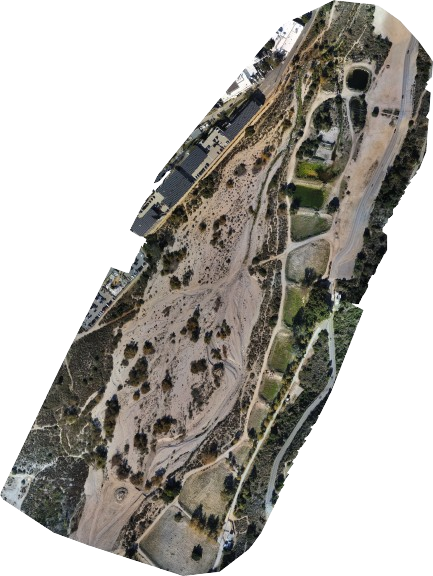
\includegraphics[scale=0.5]{images/evaluation/arroyo.png}
        \caption{Map of the Arroyo Seco area outside of the Jet Propulsion Laboratory}
    \end{figure}
    \begin{figure}
        \centering
        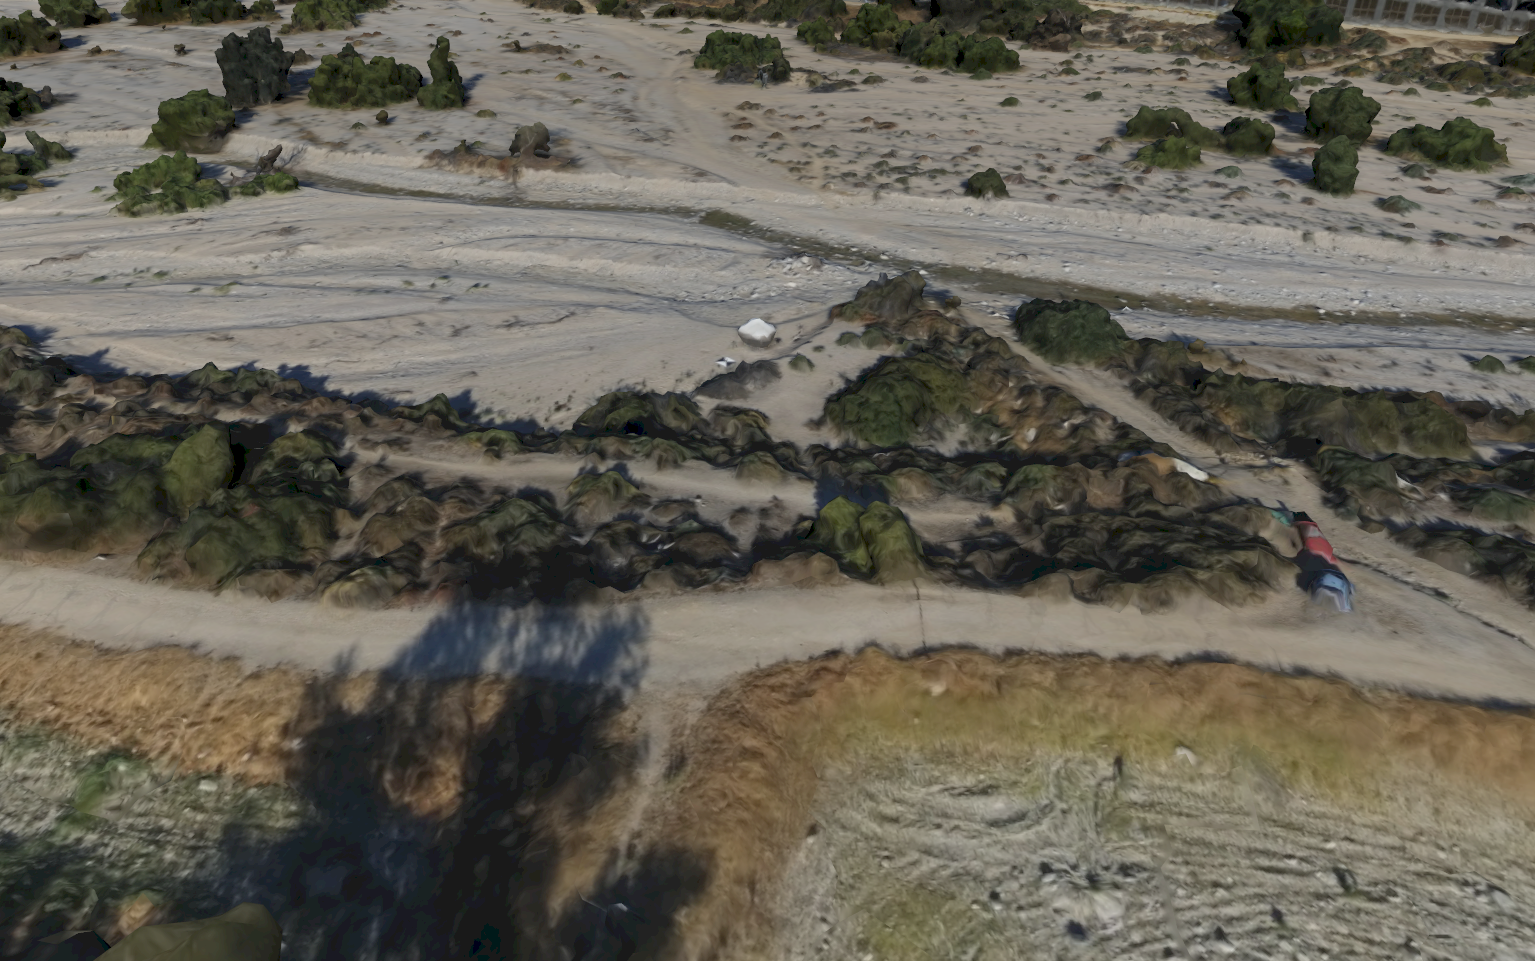
\includegraphics[scale=0.23]{images/evaluation/arroyo_map.png}
        \caption{Close Up of the Arroyo Map}
    \end{figure}
    \item Rough Test Map - A synthetically created map using Blender, designed not to have any safe landing site throughout its entire area. 
    \begin{figure}
        \centering
        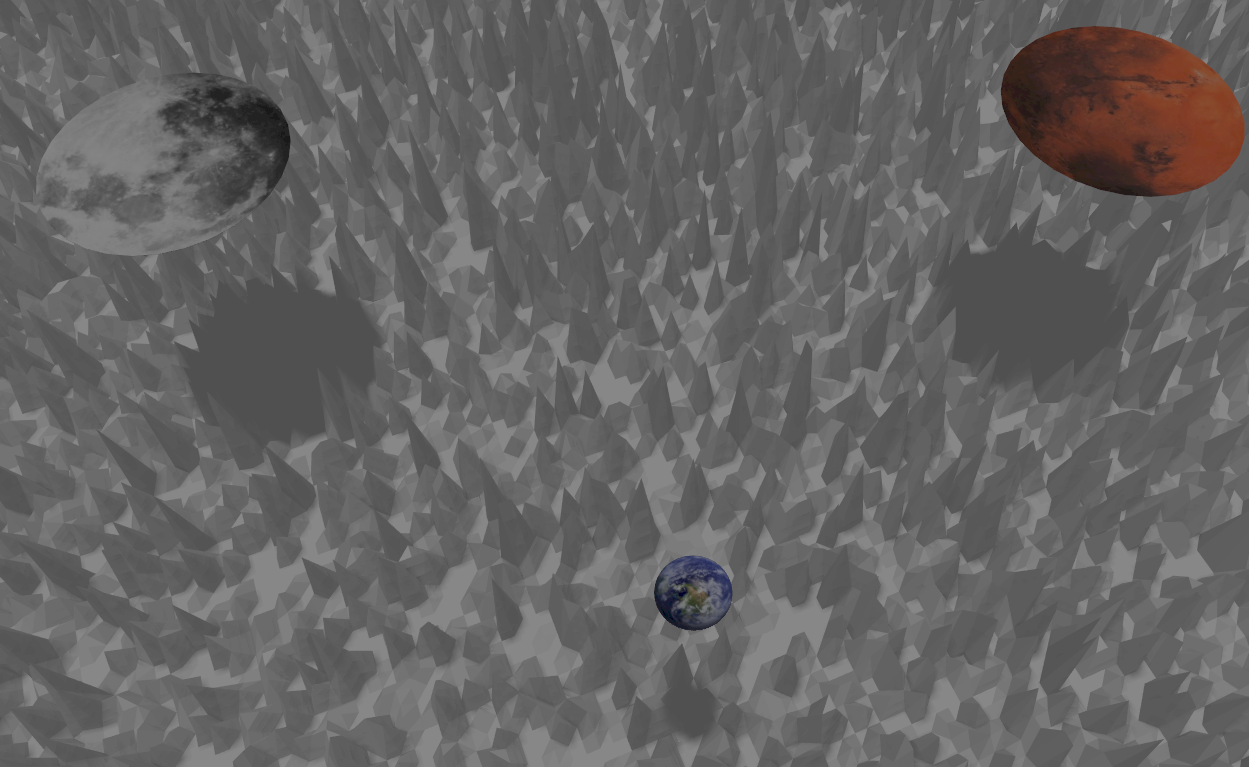
\includegraphics[scale=0.285]{images/evaluation/rough_test_map.png}
        \caption{Synthetically created map with no landing sites apart from inserted landing platforms.}
    \end{figure}
\end{itemize}
\subsection{Drone Spawn}
The drone was either spawned repetetively from a default location on the ground (The start location from when the actual fields tests were performed) or from a random location. For a simplicity way of  avoiding terrain collisions, the drone was spawned on a randomly positioned disk at 40m altitude. The start disk's size was only 0.5m in diameter which prevented it from being considered too good of a landing site by LSD. This is important because the platform implicitly gains quality due to the fact, that it is located higher up than the terrain, leading to a lower distance to the drone when flying at mission altitude.
\begin{figure}
    \centering
    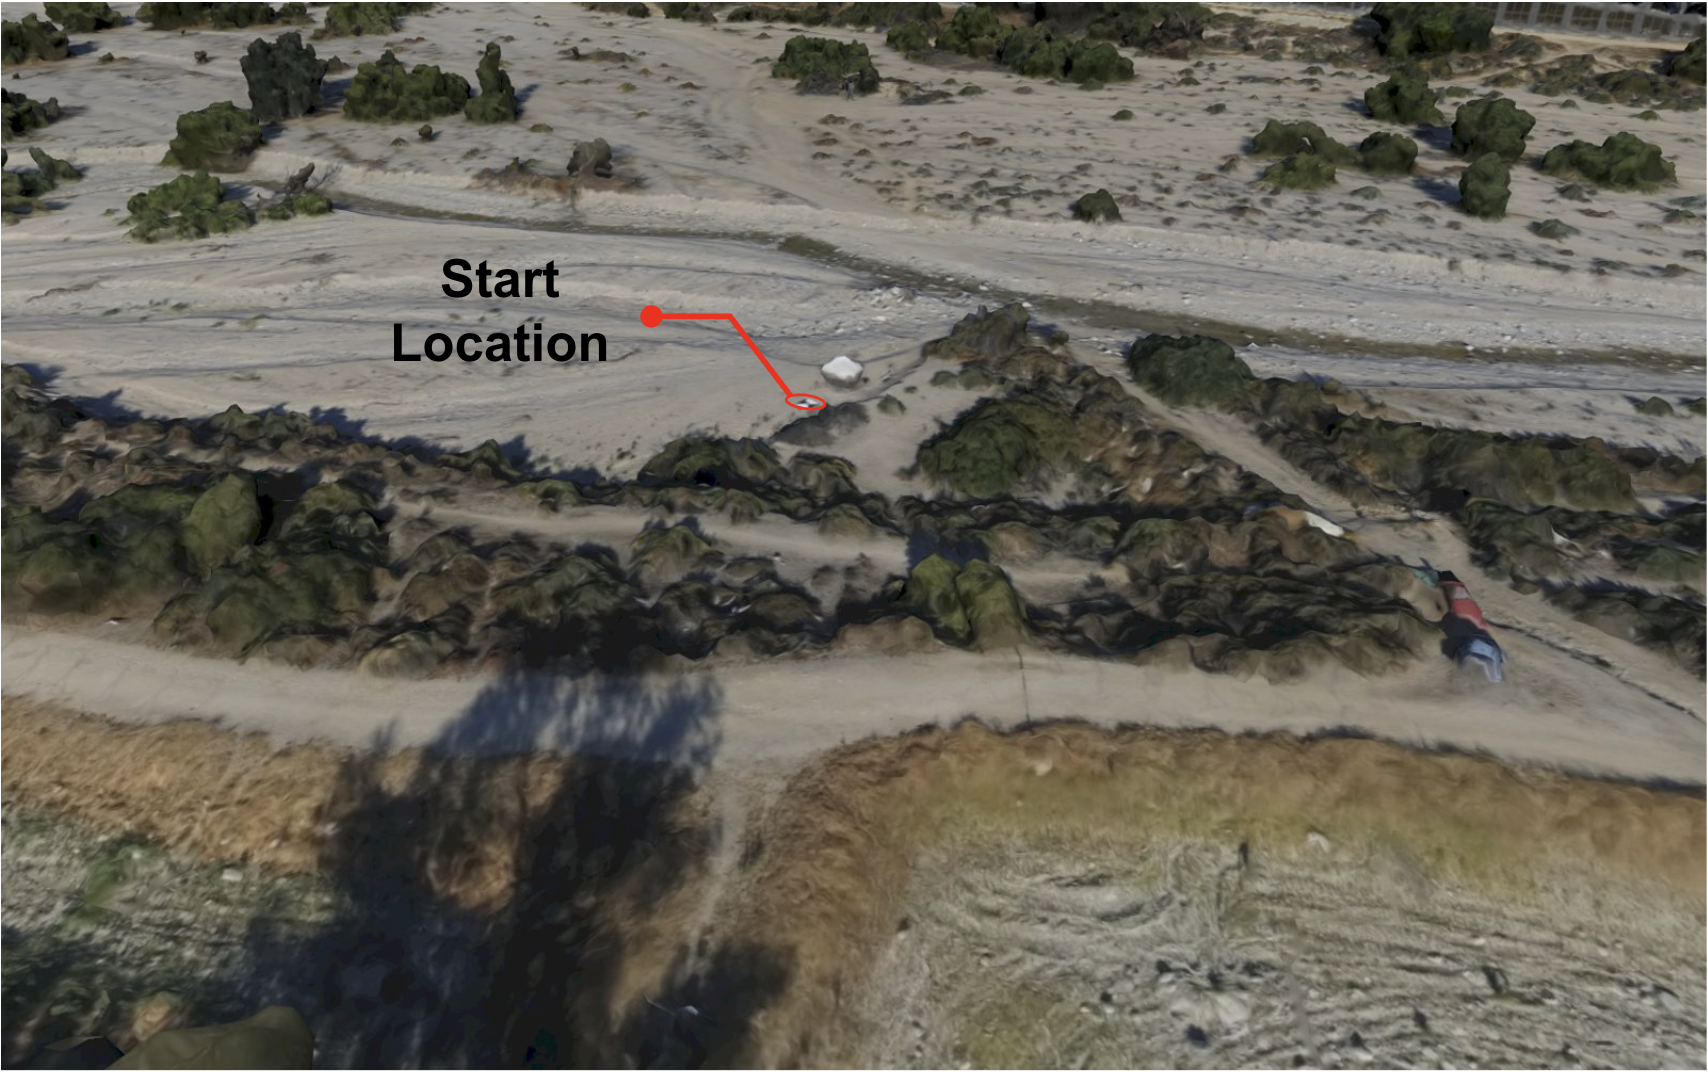
\includegraphics[scale=0.42]{images/evaluation/arroyo_with_start.png}
    \caption{Arroyo Map with Fixed Start Position}
\end{figure}
\begin{figure}
    \centering
    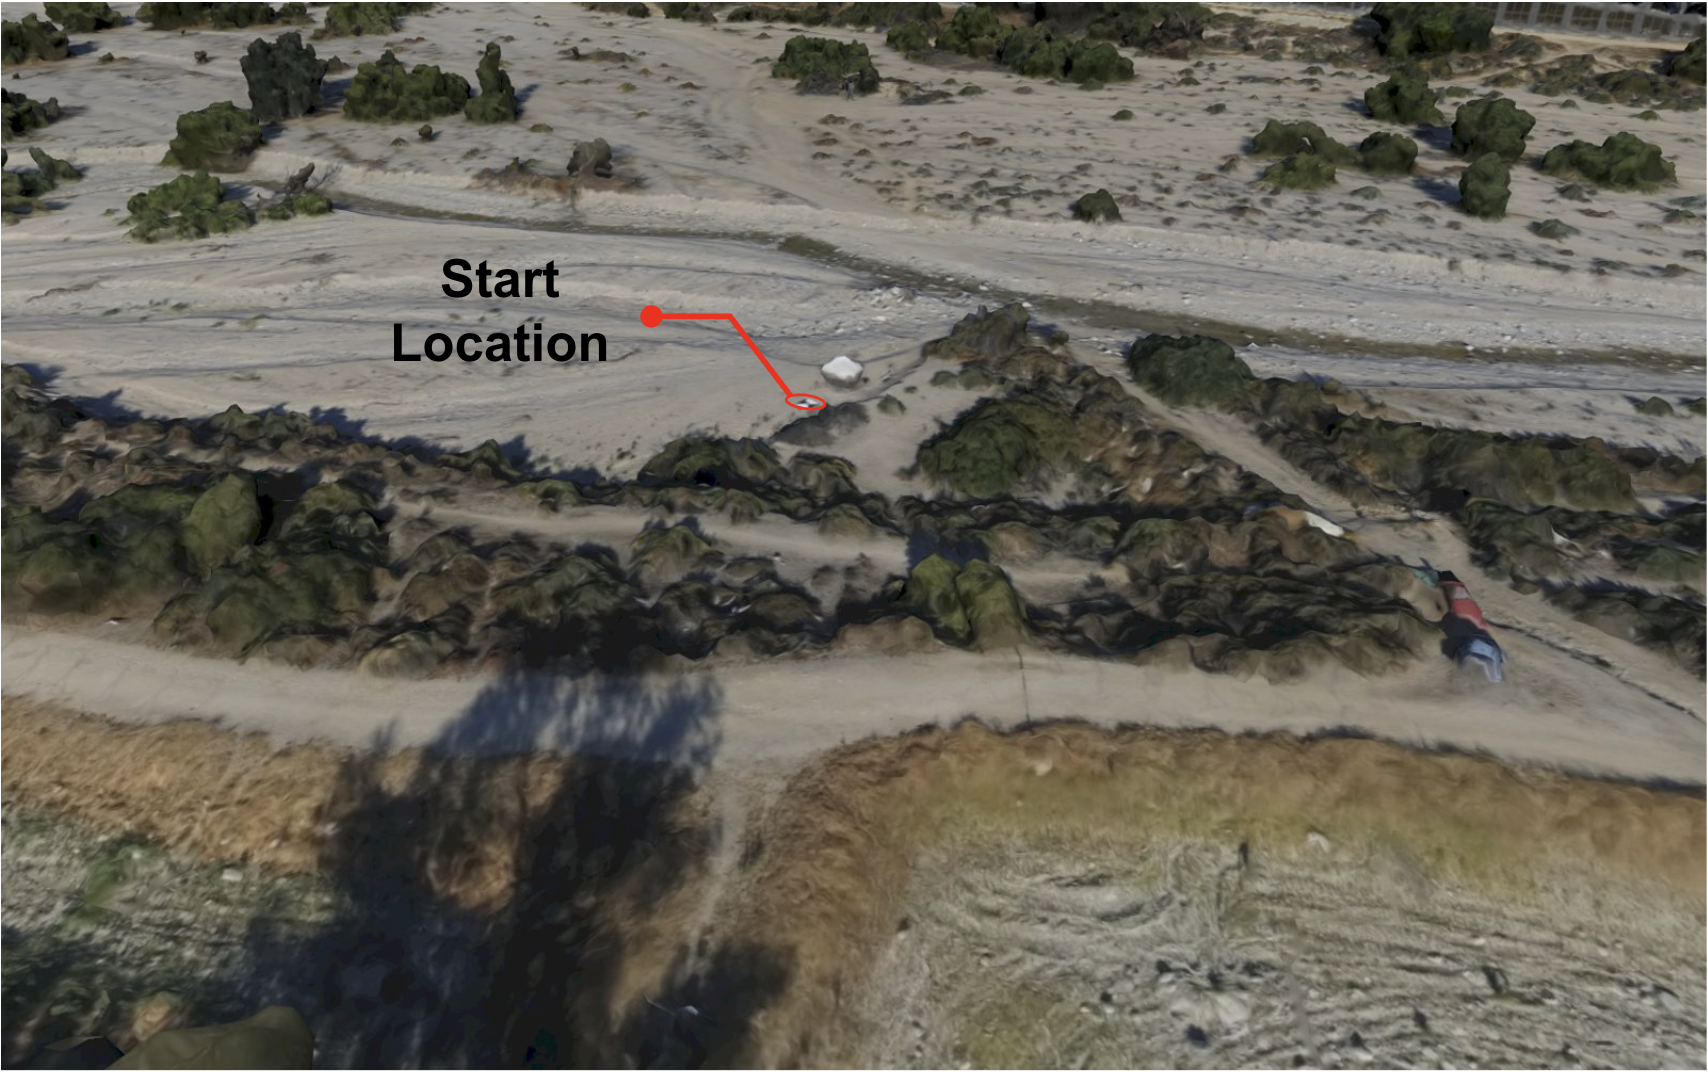
\includegraphics[scale=0.42]{images/evaluation/arroyo_with_start.png}
    \caption{Arroyo map with randomly positioned spawn platform}
\end{figure}

\subsection{Success Conditions}
To determine whether a flight was successful or not, two main metrics were considered. First of all whether the landing action in the autonomy was initiated (this happens only after the landing site selection and verification were both successful) and secondly to infere the safety of the rotorcraft, a rosbag was collected and analyzed to check whether either the roll or pitch value exceeded the crash threshold.

\textbf{Note: } In practice a threshold of 1.2 radians or shortly below 70\degree proved to be an accurate decision boundary.

\subsection{Offboard Mode connection Issues}
As will be presented in the following, connection failures between the PX4 flight controller and the autonomy ocurred, leading to the deactivation of the offboard mode and therefore the loss of control of the autonomy over the rotorcraft. These issues arose most likely because the mavros connection inbetween failed to send a necessary heartbeat repeatedly and thus the connection was intercepted.

Self evidently, this did not result in a successful landing and was not counted as such. However, as these connection issues did not occur due to insufficiencies in the pipeline presented in this work, they were not considered failures of the pipeline either.
\clearpage
\section{Test Flights}
\subsection{Arroyo - 100m Randomized Waypoints}






